\definecolor{blue}{RGB}{38,139,210}
\definecolor{cyan}{RGB}{42,161,152}
\definecolor{violet}{RGB}{108,113,196}
\definecolor{red}{RGB}{220,50,47}
\definecolor{base01}{RGB}{88,110,117}
\definecolor{base02}{RGB}{7,54,66}
\definecolor{base03}{RGB}{0,43,54}

\usetikzlibrary{calc,shapes,positioning}

\chapter{Convolutional Neural Networks}\label{chap:cnn}


\begin{figure}[ht]
    \captionsetup{justification=centering}
    \centering
    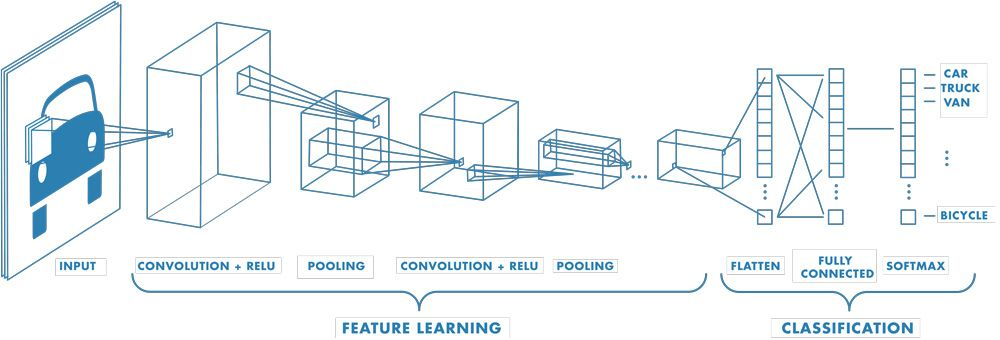
\includegraphics[width=\textwidth]{chapters/assets/cnn.jpg}
    \caption{An overview of the functioning of CNNs. Image sourced from Matlab\protect\footnotemark}
    \label{fig:cnn-overview}
\end{figure}
\footnotetext{\url{https://www.mathworks.com/discovery/convolutional-neural-network-matlab.html}}

\citeauthor{LeCun1989} proposed the novel \textbf{convolutional neural network} (CNN) architecture to tackle computer vision tasks. The specific task \citeauthor{LeCun1989} chose to solve was the recognition of handwritten digits (today a similar dataset is the MNIST\footnote{\url{http://yann.lecun.com/exdb/mnist/}} dataset). 


CNNs were originally inspired by early findings in the study of natural biological vision. They have since become the tools of choice in computer vision and as models of neural activity in visual tasks \parencite{Kuzovkin2018, Lindsay2021, Eickenberg2017}. The CNN architecture and its derivatives continue to be one of the best performing models (alongside newly the minted vision transformers \parencite{Dosovitskiy2020}) for computer vision tasks ranging from image classification to 3D depth estimation.

Even though CNNs were first introduced in \citeyear{LeCun1989}, it was AlexNet \parencite{AlexNet2012} that really launched the CNN based models into the spotlight. AlexNet outperformed its competitors by around $10\%$ on the ImageNet \parencite{deng2009imagenet} benchmark. Surpassing its competitors by such a great margin propelled AlexNet and CNNs as the dominant force in computer vision problems.


An archetypal CNN (\Cref{fig:cnn-overview}) is made up of two major components, (i) a \textbf{feature extractor} and (ii) a \textbf{classification head}. The feature extractor portion is made up of multiple convolutional layers, followed by non-linear activation functions (\Cref{sec:activation-functions}) and finally some form of \textbf{pooling} is applied.
The classification head consists of an MLP that uses the output of a feature extractor, followed by the application of the \textbf{softmax} function to get the class probabilities. We shall go over each of the operations in the following sections.


\section{Convolution}\label{sec:convolutions}

As the name implies, the basic building block of a CNN is a \textbf{convolution operator}, which we denote by an asterisk $\ast$. In its most generic form, a convolution is an operation on two functions of a real-valued argument. Suppose that we have a water-level sensor installed in a massive fish-tank. Our sensor provides a single output $x(t)$, the level of water in the tank at the time $t$. Now, our sensor is not perfect and is somewhat noisy. 
To decrease the noise in the measurements, we take averages of several measurements. The more recent the measurements, the more relevant they would be, so we would rather want this to be a weighted average that gives more importance to recent measurements.
We can achieve this by using a weighting function $w(a)$, where $a$ is the age of a given measurement. Applying the weighting function produces a new function called $S$, which provides a smooth estimate of the water level in the tank:
\begin{equation}
    \label{eqn:continous-1d-conv}
    s(t)=\int x(a) w(t-a) d a .
\end{equation}

This operation is called \textbf{convolution} and \Cref{eqn:continous-1d-conv} is often succinctly written as:
\begin{equation}
    \label{eqn:conv-1d-succinct}
    s(t) = (x \ast w)(t).
\end{equation}

In \cref{eqn:continous-1d-conv} and \cref{eqn:conv-1d-succinct} $x$ is referred to as the \textbf{input}, the function $w$ is called the \textbf{kernel}. In the terminology of the convolutional network, the output is termed \textbf{feature map}.

We can also use convolutions over multiple axes simultaneously. If we choose a two-dimensional image $I$ as input, it stands to reason that we would probably want to use a two-dimensional kernel $K$ over it:
\begin{equation}
\label{eqn:convolution-2d}
S(i, j)=(I * K)(i, j)=\sum_{m} \sum_{n} I(m, n) K(i-m, j-n).
\end{equation}

As convolution is a commutative operation, we can rewrite \Cref{eqn:convolution-2d} for a convenient implementation:
\begin{equation}
S(i, j)=(K * I)(i, j)=\sum_{m} \sum_{n} I(i-m, j-n) K(m, n).
\end{equation}

\begin{wrapfigure}{r}{0.30\textwidth}
    \centering
    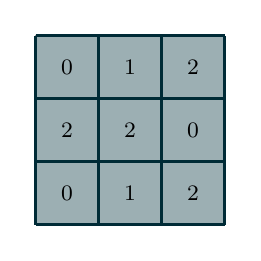
\begin{tikzpicture}[scale=.8,every node/.style={minimum size=1cm}, on grid]
        \draw[fill=base02,opacity=0.4] (0,0) rectangle (3,3);
        \draw[draw=base03,thick] (0,0) grid (3,3);
        \node (00) at (0.5,2.5) {\footnotesize 0};
        \node (01) at (1.5,2.5) {\footnotesize 1};
        \node (02) at (2.5,2.5) {\footnotesize 2};
        \node (10) at (0.5,1.5) {\footnotesize 2};
        \node (11) at (1.5,1.5) {\footnotesize 2};
        \node (12) at (2.5,1.5) {\footnotesize 0};
        \node (20) at (0.5,0.5) {\footnotesize 0};
        \node (21) at (1.5,0.5) {\footnotesize 1};
        \node (22) at (2.5,0.5) {\footnotesize 2};
\end{tikzpicture}
    \caption{A two-dimensional kernel.}
    \label{fig:2d-kernel-sample}
\end{wrapfigure}

The commutative property of convolution appears as we have \textbf{flipped} the kernel relative to the input, in the sense that as $m$ increases, the index into the input increases, but the index into the kernel decreases. While useful for mathematical proofs, its not necessary to do in terms of actual implementation. Instead, many neural network libraries implement the \textbf{cross-correlation} function, which for all intents and purposes is the same as a convolution without the kernel being flipped:
\begin{equation}
S(i, j)=(K * I)(i, j)=\sum_{m} \sum_{n} I(i+m, j+n) K(m, n).
\end{equation}\label{eqn:conv-2d-cross-correl}

An example of a two-dimensional \textit{kernel} is shown in \Cref{fig:2d-kernel-sample}, and \Cref{fig:numerical_no_padding_no_strides} shows an example of a discrete convolution using the kernel in \Cref{fig:2d-kernel-sample}. 
The blue grid is the two-dimensional input, also called the \textbf{input feature map}. In order to keep the drawing simple, a single input feature map is shown, however, it quite common to have multiple feature maps stacked on top of each other.
The kernel slides over the input feature map and, at each location, we take a product between each element of the kernel and the input element that coincides with it.
The results of the products are summarised to obtain the output at the current location (the centre of the kernel).
This process can be repeated using different kernels to generate as many \textbf{output feature maps} as required (\Cref{fig:conv-full_picture}). It must be noted that the kernel can be learnt through back-propagation.

\begin{figure}
     \centering
     \begin{subfigure}[b]{0.6\textwidth}
        \centering
        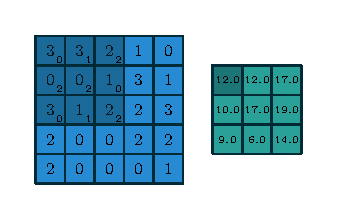
\includegraphics[width=0.32\textwidth]{chapters/assets/2d-conv-example/numerical_no_padding_no_strides_00.pdf}
        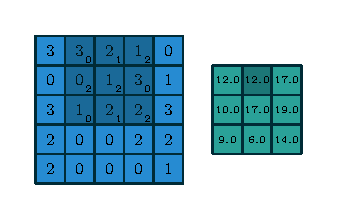
\includegraphics[width=0.32\textwidth]{chapters/assets/2d-conv-example/numerical_no_padding_no_strides_01.pdf}
        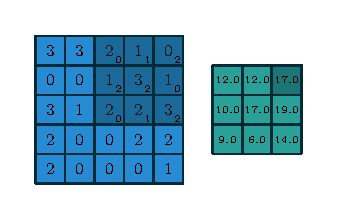
\includegraphics[width=0.32\textwidth]{chapters/assets/2d-conv-example/numerical_no_padding_no_strides_02.pdf}
        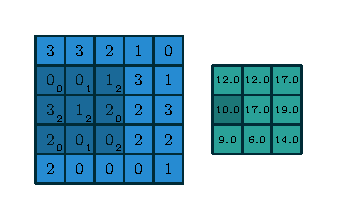
\includegraphics[width=0.32\textwidth]{chapters/assets/2d-conv-example/numerical_no_padding_no_strides_03.pdf}
        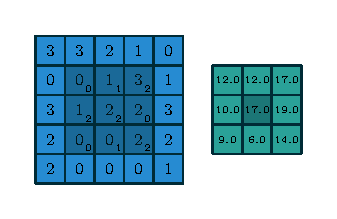
\includegraphics[width=0.32\textwidth]{chapters/assets/2d-conv-example/numerical_no_padding_no_strides_04.pdf}
        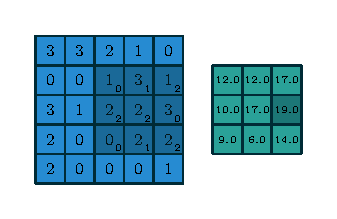
\includegraphics[width=0.32\textwidth]{chapters/assets/2d-conv-example/numerical_no_padding_no_strides_05.pdf}
        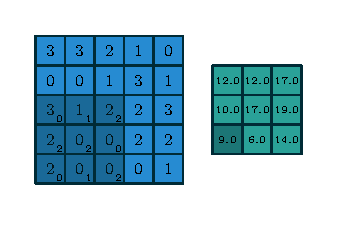
\includegraphics[width=0.32\textwidth]{chapters/assets/2d-conv-example/numerical_no_padding_no_strides_06.pdf}
        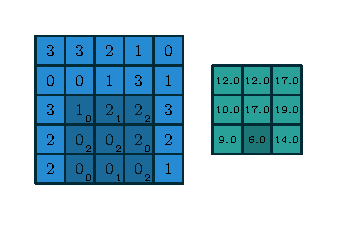
\includegraphics[width=0.32\textwidth]{chapters/assets/2d-conv-example/numerical_no_padding_no_strides_07.pdf}
        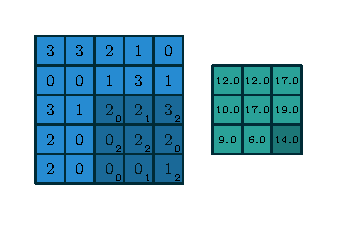
\includegraphics[width=0.32\textwidth]{chapters/assets/2d-conv-example/numerical_no_padding_no_strides_08.pdf}
        \caption{\label{fig:numerical_no_padding_no_strides} Computing the output
            values of a discrete convolution.}
     \end{subfigure}
     
     \begin{subfigure}[b]{0.6\textwidth}
        \centering
        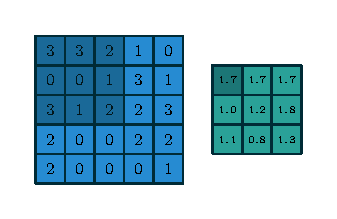
\includegraphics[width=0.32\textwidth]{chapters/assets/avg-pooling/numerical_average_pooling_00.pdf}
        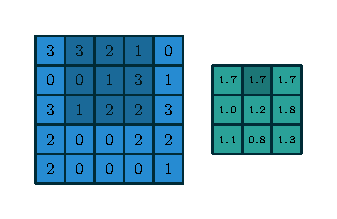
\includegraphics[width=0.32\textwidth]{chapters/assets/avg-pooling/numerical_average_pooling_01.pdf}
        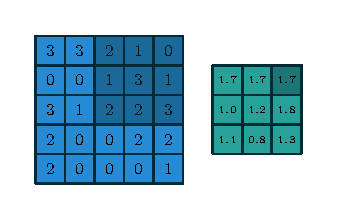
\includegraphics[width=0.32\textwidth]{chapters/assets/avg-pooling/numerical_average_pooling_02.pdf}
        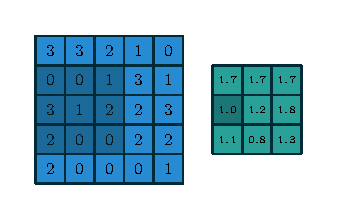
\includegraphics[width=0.32\textwidth]{chapters/assets/avg-pooling/numerical_average_pooling_03.pdf}
        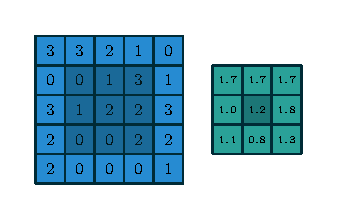
\includegraphics[width=0.32\textwidth]{chapters/assets/avg-pooling/numerical_average_pooling_04.pdf}
        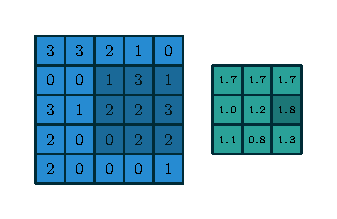
\includegraphics[width=0.32\textwidth]{chapters/assets/avg-pooling/numerical_average_pooling_05.pdf}
        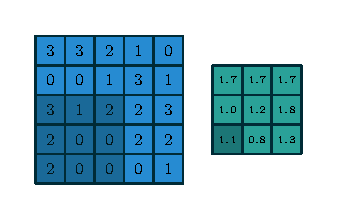
\includegraphics[width=0.32\textwidth]{chapters/assets/avg-pooling/numerical_average_pooling_06.pdf}
        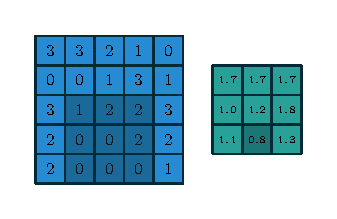
\includegraphics[width=0.32\textwidth]{chapters/assets/avg-pooling/numerical_average_pooling_07.pdf}
        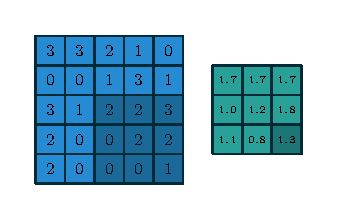
\includegraphics[width=0.32\textwidth]{chapters/assets/avg-pooling/numerical_average_pooling_08.pdf}
        \caption{\label{fig:numerical_average_pooling} Computing the output values
            of a $3 \times 3$ average pooling operation on a $5 \times 5$ input
            using $1 \times 1$ strides.}
     \end{subfigure}
     \caption{Examples of convolution and average pooling operations \parencite{Dumoulin2016}.}
     \label{fig:conv-and-avg-pool}
\end{figure}


\begin{figure}[bt]
    \centering
    \captionsetup{justification=RaggedRight}
    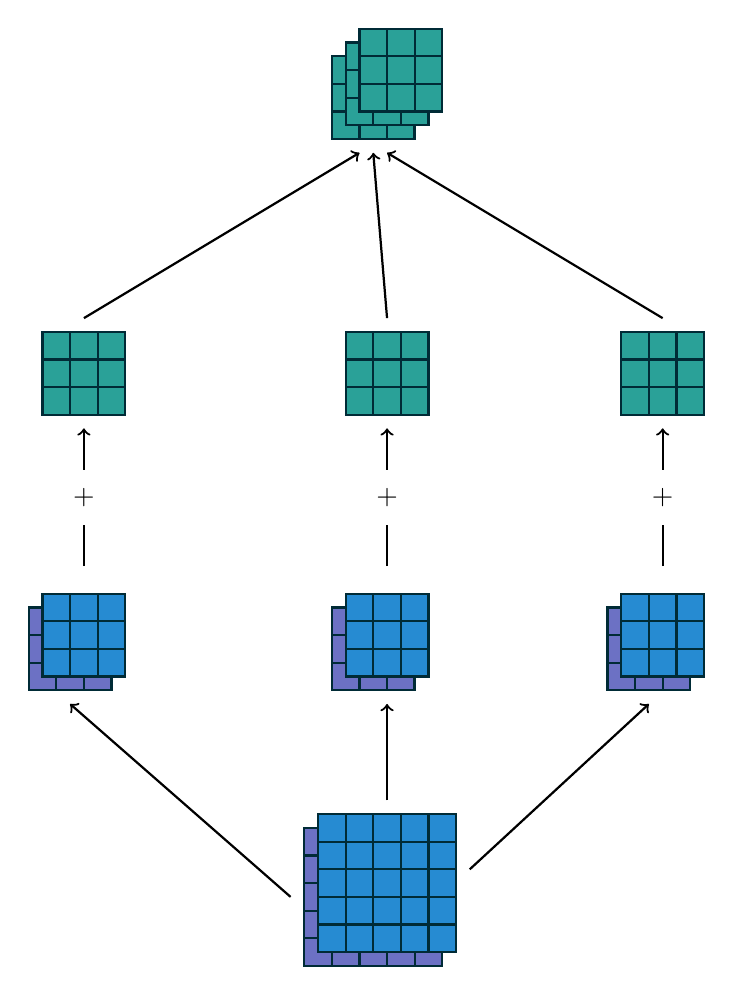
\begin{tikzpicture}[scale=.35,every node/.style={minimum size=1cm}, on grid]
    \begin{scope}[xshift=0cm,yshift=0cm]
        \begin{scope}[xshift=0cm,yshift=0cm]
            \draw[draw=base03,fill=violet,thick]
                (0,0) grid (5,5) rectangle (0,0);
        \end{scope}
        \begin{scope}[xshift=0.5cm,yshift=0.5cm]
            \draw[draw=base03,fill=blue,thick]
                (0,0) grid (5,5) rectangle (0,0);
        \end{scope}
    \end{scope}
    \foreach \x in {-10,1,11} {%
        \begin{scope}[xshift=\x cm,yshift=10cm]
            \begin{scope}[xshift=0cm,yshift=0cm]
                \draw[draw=base03,fill=violet,thick]
                    (0,0) grid (3,3) rectangle (0,0);
            \end{scope}
            \begin{scope}[xshift=0.5cm,yshift=0.5cm]
                \draw[draw=base03,fill=blue,thick]
                    (0,0) grid (3,3) rectangle (0,0);
            \end{scope}
        \end{scope}
        \begin{scope}[xshift=\x cm,yshift=20cm]\begin{scope}[xshift=0.5cm]
            \draw[draw=base03,fill=cyan,thick]
                (0,0) grid (3,3) rectangle (0,0);
        \end{scope}\end{scope}
    }
    \begin{scope}[xshift=1cm,yshift=30cm]
        \foreach \s in {0.0,0.5,1.0} {%
            \begin{scope}[xshift=\s cm,yshift=\s cm]
                \draw[draw=base03,fill=cyan,thick]
                    (0,0) grid (3,3) rectangle (0,0);
            \end{scope}
        }
    \end{scope}
    \draw[->, thick] (-0.5,2.5) to (-8.5,9.5);
    \draw[->, thick] (3,6) to (3,9.5);
    \draw[->, thick] (6,3.5) to (12.5,9.5);
    \draw[thick]  (-8,14.5) to (-8,16);
    \draw[->, thick]  (-8,18) to (-8,19.5);
    \node[thick] (p1) at (-8,17) {$+$};
    \draw[thick]  (3,14.5) to (3,16);
    \draw[->, thick]  (3,18) to (3,19.5);
    \node[thick] (p2) at (3,17) {$+$};
    \draw[thick]  (13,14.5) to (13,16);
    \draw[->, thick]  (13,18) to (13,19.5);
    \node[thick] (p3) at (13,17) {$+$};
    \draw[->, thick]  (-8,23.5) to (2,29.5);
    \draw[->, thick]  (3,23.5) to (2.5,29.5);
    \draw[->, thick]  (13,23.5) to (3,29.5);
\end{tikzpicture}
    \caption{\label{fig:conv-full_picture} A convolution mapping from two input
        feature maps to three output feature maps using a $3 \times 2 \times 3
        \times 3$ collection of kernels $\symbf{w}$. In the left pathway, input
        feature map 1 is convolved with kernel $\symbf{w}_{1,1}$ and input
        feature map 2 is convolved with kernel $\symbf{w}_{1,2}$, and the
        results are summed together elementwise to form the first output feature
        map. The same is repeated for the middle and right pathways to form the
        second and third feature maps, and all three output feature maps are
        grouped together to form the output. Figure courtesy \textcite{Dumoulin2016}.}
\end{figure}


\section{Pooling}\label{sec:conv-pooling}

In addition to convolution operation described in \cref{sec:convolutions}, \textbf{pooling} operations make up another important aspect of a CNN. Pooling operations are meant to reduce the size of the feature maps by using some function to \textbf{summarise} regions of the feature map, such as taking the average or maximum value of a collection of values in a feature map present in a window.

Pooling operations work similarly to a convolution by sliding a window across the input and applying a pooling function to the contents of the window. 
Pooling operations replace the linear combination described by the kernel with some other function. \Cref{fig:numerical_average_pooling} shows an example of the \textbf{average pooling} operation, which applies the averaging function on the contents of the sliding window. Similarly, \textbf{maximum pooling} is another pooling operation that takes the maximum of the content present in the sliding window.


\newpage
\section{Kernels as Feature Extractors}\label{sec: kernel-feature-extractor}
Each convolutional layer is characterised by the size of the kernels, the number of kernels, the padding and \textbf{stride}; the relationship between these components is not trivial to intuitively infer. Every kernel's weights act as a particular feature detector, and thus learning the kernel's weights translates into learning the features. \Cref{fig:feature-viz} shows the types of features and patterns learnt by a fully trained model in various layers. Note that as the number of layers increases, the network is learning more and more specific and complex patterns.

\begin{figure}[ht]
    \centering
    \captionsetup{justification=RaggedRight}
    \includegraphics[scale=0.6]{chapters/assets/rob3_new6.pdf}
    \caption{Visualisation of features learnt in various layers by a fully trained CNN. Image from \textcite{Zeiler2013}.}
    \label{fig:feature-viz}
\end{figure}